% Condensed Sections 3--4: the tactical contribution is kept explicit, while
% standard execution details are summarized to preserve experimental space.

% =====================================================================
\section{Game-Guided Tactical Corridor Policy}\label{sec:tactical}
% =====================================================================

The proposed method separates interaction reasoning from dynamic execution by
placing a time-varying feasible corridor at their interface.  This choice is
deliberate.  A discrete maneuver label does not specify the lateral space that
the planner may use, a target point does not preserve feasibility between
updates, and a single learned trajectory couples tactical prediction to one
particular downstream solver.  In contrast, the corridor exposes the tactical
decision as explicit Frenet inequalities while allowing the common path,
speed, and control modules to determine how the maneuver is executed.  The
method has three coupled elements.  First, a Stackelberg--IBR model assigns
interaction-aware value to candidate feasible sets.  Second, a distributional
actor--critic amortizes that game and maps the current duel and track preview
to corridor parameters.  Third, persistent hybrid logic converts each policy
sample into temporally consistent bounds.  The following subsections describe
these elements in the same order as the online information flow.

\subsection{Stackelberg--IBR feasible-set decision}
\label{subsec:game_formulation}

The learned decision is a planner-compatible feasible set rather than a
steering or longitudinal command.  At tactical step $t$, the encoder combines
ego and opponent states, track preview, the current mode, and the locked pass
side.  The policy action is projected onto admissible bounds; a deterministic
finite-state machine (FSM) and corridor carver then publish
\begin{equation}
\begin{aligned}
\widetilde{\bm o}_t&=\mathcal E(\bm x_{e,t},\bm x_{o,t},\mathcal P,
 m_t,\sigma_t^{\rm lock}),\\
\bm a_t&=\Pi_{\mathcal A}\!\left(\pi_\theta(\widetilde{\bm o}_t)\right),
\quad (m_{t+1},\sigma_{t+1}^{\rm lock})=\mathcal F_m(\bm a_t,\bm o_t),\\
\mathcal G_t&=\bigl(m_{t+1},\sigma_{t+1}^{\rm lock},V_{{\rm cap},t},
\mathcal C_t\bigr),\quad
\mathcal C_t=\mathcal F_c(\mathcal B,\bm x_{o,t},\bm a_t,m_{t+1}),
\end{aligned}
\label{eq:tactical_stack}
\end{equation}
where $\mathcal B(s)=[n_{\rm trk}^-(s),n_{\rm trk}^+(s)]$ and
$\mathcal C_t=\{(s,n):n_t^-(s)\le n\le n_t^+(s)\}$.  Only
$\pi_\theta$ is learned; projection, mode persistence, footprint exclusion,
and corridor filtering are deterministic and independently inspectable.
Equation~\eqref{eq:tactical_stack} is therefore an interface contract: the
policy may change the side preference, usable width, clearance, and speed cap,
but it cannot bypass the track boundary or directly alter an actuator.  The
contract also makes tactical alternatives comparable before a path is chosen.
Two actions can reserve different sides or recovery margins even when their
short-horizon centre trajectories appear similar, which is important near an
opponent where locally smooth trajectories can imply very different future
passing options.

The interaction prior is obtained from a leader--follower game.  For vehicle
$i$, a hybrid action contains a maneuver/side choice $d_i$ and continuous
aggressiveness/preference variables $c_i$.  Its utility collects progress,
relative race position, safety, terminal recoverability, and action
regularity in one expression,
\begin{equation}
U_i=w_i^p\Phi_i^p+w_i^r\Phi_i^r-w_i^s\Phi_i^s
    +w_i^t\Phi_i^t-w_i^c\Phi_i^c .
\label{eq:utility_decomposition}
\end{equation}
For a fixed discrete profile, the opponent response is approximated by
iterative best response (IBR), and the ego selects the worst-case value in a
local response neighborhood:
\begin{equation}
\begin{aligned}
c_i^{(\nu+1)}&\in\argmax_{c_i\in\mathcal C_i(d_i)}
 U_i(d,c_e,c_i,c_{-i}^{(\nu)}),\\
\bm a_{\rm th}^{\star}(\bm o)&\in
\argmax_{(d_e,c_e)\in\mathcal A_e^{\rm safe}(\bm o)}
\min_{\|c_{-e}-c_{-e}^{\rm IBR\star}\|\le\delta}
U_e((d_e,c_e),(d_{-e},c_{-e})).
\end{aligned}
\label{eq:ibr_decision}
\end{equation}
This game is evaluated during training to generate structural targets.  The
online actor amortizes repeated IBR solutions and therefore preserves the
interaction semantics without placing an equilibrium solver in the real-time
control loop.
The construction transfers three pieces of structure rather than treating the
game as an independent expert: $\bm a_{\rm th}^{\star}$ supplies an action
prior, the robust inner minimum supplies a value target, and the decomposition
of $U_i$ determines the roles represented in the closed-loop reward.  Thus the
game specifies which corridor is strategically useful, whereas learning
compresses repeated solutions into a fixed-cost forward pass.  This division
also creates a direct ablation hook: removing game guidance changes the
tactical supervision without changing the policy interface or executor.

Physical admissibility acts on all tactical candidates without defining their
strategic value. A short preview of a candidate corridor and speed cap gives
tangential and normal acceleration demands
$(\widehat a_{T,t,k},\widehat a_{N,t,k})$. With the load-dependent limits of
Section~\ref{sec:model}, the common projection set is
\begin{equation}
\begin{aligned}
\widehat\rho_{t,k}(\bm a)&=
\left|\frac{\widehat a_{N,t,k}}{a_N^{\max}(\widehat V_{t,k})}\right|^p+
\left|\frac{\widehat a_{T,t,k}}{a_T^{\max}(\widehat V_{t,k})}\right|^p,\\
\mathcal A_e^{\rm safe}(\widetilde{\bm o}_t)&=
\left\{\bm a\in\mathcal A_e:\max_k\widehat\rho_{t,k}(\bm a)\le1\right\}.
\end{aligned}
\label{eq:tire_safe_action}
\end{equation}
An out-of-set candidate is projected or its $V_{\rm cap}$ is reduced before
game or critic evaluation. This step links the learned corridor to the vehicle
model in Fig.~\ref{fig:tire_characteristics}; it does not choose the passing
side or replace the interaction utility.

\subsection{Game-guided distributional policy}
\label{subsec:theory_guided_rl}

The input is a 51-dimensional vector
$\widetilde{\bm o}_t=[\bm o_t^{\rm duel},\bm\rho(s_e),\bm\rho(s_o)]$:
$\bm o_t^{\rm duel}\in\mathbb R^{27}$ contains normalized ego/opponent
kinematics, relative progress and lateral gap, closing-time features, FSM
memory, and race status; each $\bm\rho\in\mathbb R^{12}$ contains curvature
and usable-width statistics over a 300-m preview.  The actor produces the
ten physical parameters
\begin{equation}
\bm a_t=\bigl[L_t^{\rm cap},R_t^{\rm cap},d_{\rm safe},V_{\rm cap},
g_{\rm chase},g_{\rm ot},g_{\rm abort},b_{\rm lat},w_{\rm safe},q_{\rm side}
\bigr]^\top,
\label{eq:action_vec}
\end{equation}
which respectively control lateral capacity, clearance, speed, hysteresis,
far-field bias, recovery width, and pass side.  A tanh output is affinely
scaled to the intervals in Table~\ref{tab:tactical_settings} in
\ref{app:parameters};
$\Pi_{\mathcal A}$ enforces ordered gap thresholds and a non-degenerate
corridor before the action reaches the FSM.

The reward mirrors Eq.~\eqref{eq:utility_decomposition} but is evaluated from
closed-loop events and geometry,
\begin{equation}
\begin{aligned}
r_t={}&w_{\rm ot}r_{\rm ot}+w_{\rm ovb}r_{\rm ovb}
      +w_{\rm col}r_{\rm col}+w_{\rm lat}r_{\rm lat}\\
&+w_{\rm crush}r_{\rm crush}+w_{\rm app}r_{\rm app}
      +w_{\rm sm}r_{\rm sm}+w_{\rm gs}r_{\rm gs}\\
&+w_{\rm sbs}r_{\rm sbs}+w_{\rm wide}r_{\rm wide}.
\end{aligned}
\label{eq:reward_sum}
\end{equation}
The terms encode pass/overtaken events, contact, lateral feasibility, corridor
collapse, approach progress, action and corridor smoothness, side-by-side
clearance, and retained usable width.  Their reported weights are listed in
Table~\ref{tab:tactical_settings} rather than expanded into routine feature
formulae in the main text.

Truncated Quantile Critics (TQC) model the return distribution and remove the
largest target atoms before the Bellman backup. This directly addresses the
optimistic estimates induced by a small number of high-return passes, whereas
the game supplies interaction structure that a scalar environment reward does
not encode explicitly. To keep actor and critic evaluation consistent with the
shared physical admissibility check, the raw next action is projected by
Eq.~\eqref{eq:tire_safe_action} before the target critics are evaluated,
\begin{equation}
\begin{aligned}
\widetilde{\bm a}_{t+1}&\sim
\pi_\theta(\cdot\mid\widetilde{\bm o}_{t+1}),\\
\bm a_{t+1}^{\rm F}&=\Pi_{\mathcal A_e^{\rm safe}}
(\widetilde{\bm a}_{t+1}),\\
\ell_{t+1}&=\log\pi_\theta(\widetilde{\bm a}_{t+1}
\mid\widetilde{\bm o}_{t+1}),\\
\mathcal Y_t&=\left\{r_t+\gamma\left[
z_{(k)}'(\widetilde{\bm o}_{t+1},\bm a_{t+1}^{\rm F})
-\alpha\ell_{t+1}\right]\right\}_{k=1}^{K},\quad K<2N_q .
\end{aligned}
\label{eq:tqc_truncated_target}
\end{equation}
The online actor loss likewise evaluates the critics at the projected action,
and the projected mean $\mu_\theta^{\rm F}=\Pi_{\mathcal A_e^{\rm safe}}
(\mu_\theta)$ is used for game-prior alignment.  Thus high return cannot be
assigned to a speed--corridor combination solely by extrapolating beyond the
tire-force support represented in Section~\ref{sec:model}.
Discarding the upper tail limits optimistic backups caused by rare, high-return
passing sequences, while retaining a distribution rather than a single mean
allows the critic to distinguish corridors with similar expected progress but
different adverse-return profiles.  This is useful in racing interactions,
where a small number of late or geometrically interlocked commitments can
dominate the outcome of an otherwise fast policy.  The training objective adds
two game-derived signals to the standard quantile-Huber critic and
entropy-regularized actor losses:
\begin{equation}
\begin{aligned}
\mathcal L={}&J_Q(\varphi)+\lambda_\pi J_\pi(\theta)
 +\lambda_p\|\mu_\theta^{\rm F}(\widetilde{\bm o})-
 \bm a_{\rm th}^{\star}(\widetilde{\bm o})\|_{W_c}^{2}\\
&+\lambda_g\bigl(\widehat{\mathcal G}_\psi(\widetilde{\bm o},\bm a)
-\underline{\mathcal V}_e(\bm a\mid\widetilde{\bm o})\bigr)^2 .
\end{aligned}
\label{eq:total_loss}
\end{equation}
The first added term aligns the actor mean with the IBR action, emphasizing
safety-critical components through $W_c$; the second anchors an auxiliary
head to the robust game value.  These terms are used only for training.  The
deployed actor has the same 51-to-10 interface in every scenario.  Network,
replay, quantile, and target-update settings are reported in
Tables~\ref{tab:setup_params} and~\ref{tab:tactical_settings} in
\ref{app:parameters}.
Consequently, game guidance shapes both the action and value representations
during learning, whereas truncation controls return overestimation within the
off-policy update.  The two mechanisms are complementary: the former supplies
interaction structure and the latter controls distributional optimism.  At
deployment, neither adds an iterative solver or an auxiliary prediction call
to the tactical update.

\subsection{Persistent intention and corridor synthesis}
\label{subsec:corridor_synthesis}

The FSM converts each continuous policy sample into a temporally persistent
intent.  Its nominal modes are \textsc{Raceline}, \textsc{Shadow},
\textsc{Overtake}, \textsc{Hold}, and \textsc{Defend}.  A side may be locked
only when opponent-excluded width and relative-speed gates are both satisfied;
the lock is retained throughout the duel.  The complete online conversion is
summarized in Algorithm~\ref{alg:tactical_corridor}.

At station $s_k$, the carver first intersects the action-capped track interval
with the mode-dependent opponent exclusion.
{\color{blue}
\begin{equation}
\begin{aligned}
\rho_{n,j,k}
&=\frac{1}{2}\left(
L_j|\sin\xi_{j,k}|+W_j|\cos\xi_{j,k}|
\right),\quad j\in\{e,o\},\\
\rho_{{\rm exc},k}
&=\rho_{n,e,k}+\rho_{n,o,k}+d_{\rm safe},\\
\widehat n_{t,k}^{-}
&=\begin{cases}
\max\!\left\{n_{{\rm cap},k}^{-},
n_{o,k}+\eta_k\rho_{{\rm exc},k}\right\},
&\sigma_t^{\rm lock}=+1,\\
n_{{\rm cap},k}^{-},&\sigma_t^{\rm lock}=-1,
\end{cases}\\
\widehat n_{t,k}^{+}
&=\begin{cases}
n_{{\rm cap},k}^{+},&\sigma_t^{\rm lock}=+1,\\
\min\!\left\{n_{{\rm cap},k}^{+},
n_{o,k}-\eta_k\rho_{{\rm exc},k}\right\},
&\sigma_t^{\rm lock}=-1.
\end{cases}
\end{aligned}
\label{eq:core_overtake_carver}
\end{equation}
}
\textcolor{blue}{Here
$[n_{{\rm cap},k}^{-},n_{{\rm cap},k}^{+}]$ denotes the track interval after
applying $L_t^{\rm cap}$ and $R_t^{\rm cap}$, and
$(L_j,W_j,\xi_{j,k})$ are the dimensions and heading error of vehicle $j$.
Accordingly, $\rho_{n,e,k}$ and $\rho_{n,o,k}$ are the projected lateral
half-widths, while $d_{\rm safe}$ is the policy-specified additional clearance.
The factor $\eta_k\in[0,1]$ combines the existing longitudinal fade and ramp,
vanishing outside the opponent influence interval and approaching one as the
ego vehicle approaches.  Because positive $n$ follows the left normal in
Eq.~\eqref{eq:frenet_frame}, $\sigma_t^{\rm lock}=+1$ raises the lower bound
for a left-side pass, while $\sigma_t^{\rm lock}=-1$ lowers the upper bound for
a right-side pass.  Equation~\eqref{eq:core_overtake_carver} describes only the
core \textsc{Overtake} contraction; \textsc{Shadow}, \textsc{Hold}, and
\textsc{Defend} retain the biases in Algorithm~\ref{alg:tactical_corridor}.
The existing minimum-width check and exponential moving-average filter are
applied afterward, and this carver relation is not a formal safety guarantee.}
If the raw interval
$[\widehat n_{t,k}^-,\widehat n_{t,k}^+]$ satisfies the minimum-width gate, its
bounds are filtered as
\begin{equation}
n_{t,k}^{\pm}=\beta n_{t-1,k}^{\pm}
 +(1-\beta)\widehat n_{t,k}^{\pm},\qquad
\widehat n_{t,k}^+-\widehat n_{t,k}^-\ge L_{\min}^{\rm corr};
\label{eq:corridor_filter}
\end{equation}
otherwise the update is rejected and the last feasible corridor is retained.
The minimum-width condition protects the path solver from a geometrically
empty request, while the filter suppresses update-to-update boundary motion.
These spatial checks complement the FSM's temporal hysteresis: the former
preserve an executable interval at each station, and the latter prevents the
selected interval from alternating between passing sides during one duel.

\begin{algorithm}[!tbp]
\caption{Persistent tactical-corridor update}
\label{alg:tactical_corridor}
\begin{algorithmic}[1]
\REQUIRE $\mathcal B$, ego/opponent states, previous $(m,\sigma^{\rm lock},
\mathcal C)$, map preview $\mathcal P$
\STATE Encode $\widetilde{\bm o}$; sample and project
$\bm a\leftarrow\Pi_{\mathcal A}(\pi_\theta(\widetilde{\bm o}))$
\STATE Compute relative gap, closing condition, and free width on each side
\IF{inside overtake gate and selected side is geometrically ready}
  \STATE set $m\leftarrow\textsc{Overtake}$ and lock the selected side
\ELSIF{inside chase gate}
  \STATE set $m\leftarrow\textsc{Shadow}$
\ELSIF{abort or post-pass condition is active}
  \STATE set $m\leftarrow\textsc{Hold}$
\ELSE
  \STATE select \textsc{Raceline}/\textsc{Defend} from front/rear race state
\ENDIF
\STATE Initialize each station from track bounds capped by
$L^{\rm cap},R^{\rm cap}$
\STATE Exclude the opponent footprint enlarged by $d_{\rm safe}$; apply the
mode/side bias and $V_{\rm cap}$
\STATE Reject corridors narrower than $L_{\min}^{\rm corr}$; otherwise apply
the exponential moving-average filter
\RETURN $\mathcal G=(m,\sigma^{\rm lock},V_{\rm cap},\mathcal C)$
\end{algorithmic}
\end{algorithm}

\begin{figure}[!tbp]
\centering
\subfloat[\textsc{Raceline}/\textsc{Hold}.]{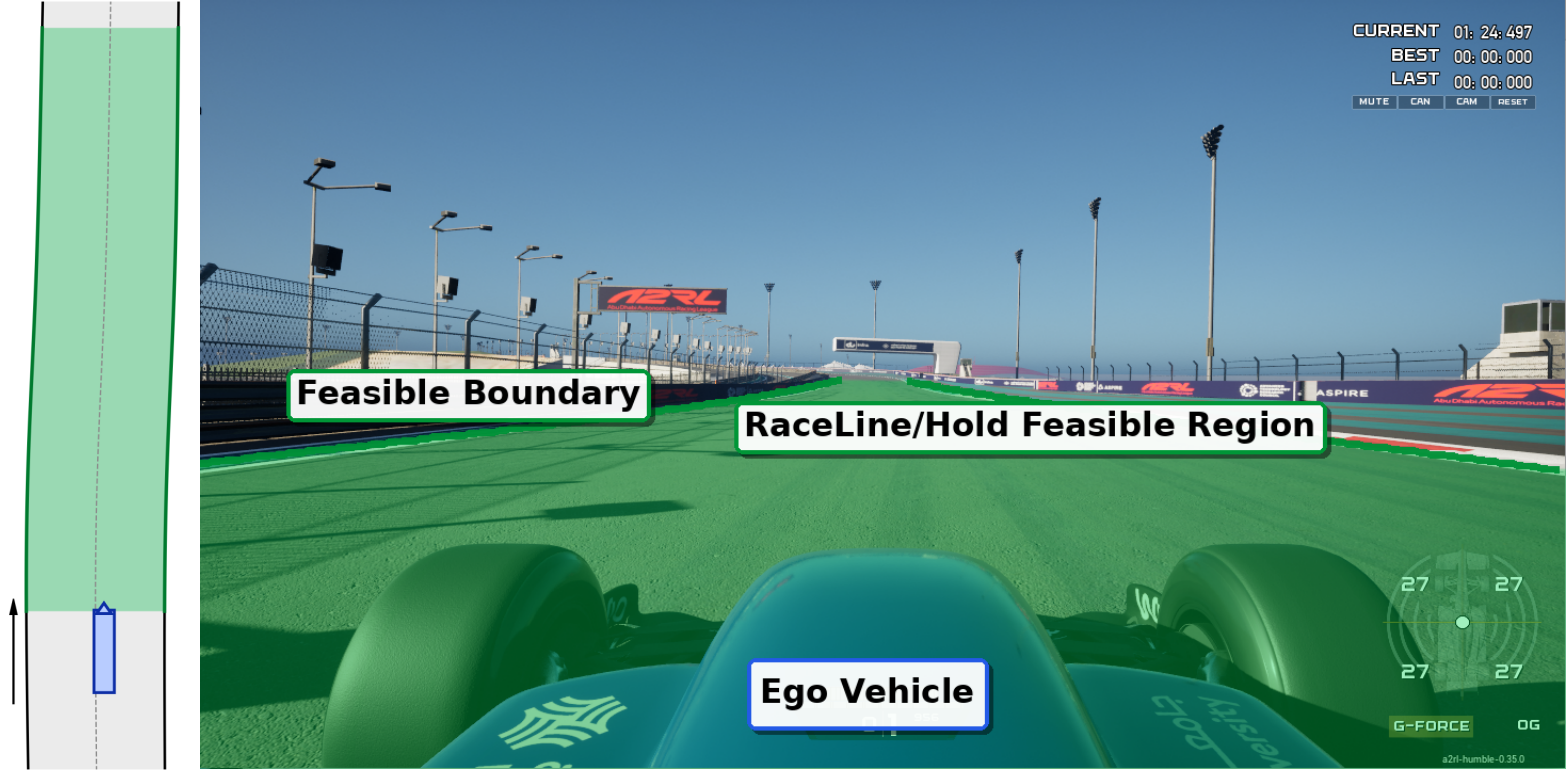
\includegraphics[width=0.48\linewidth]{race.png}}
\hfill
\subfloat[\textsc{Shadow}.]{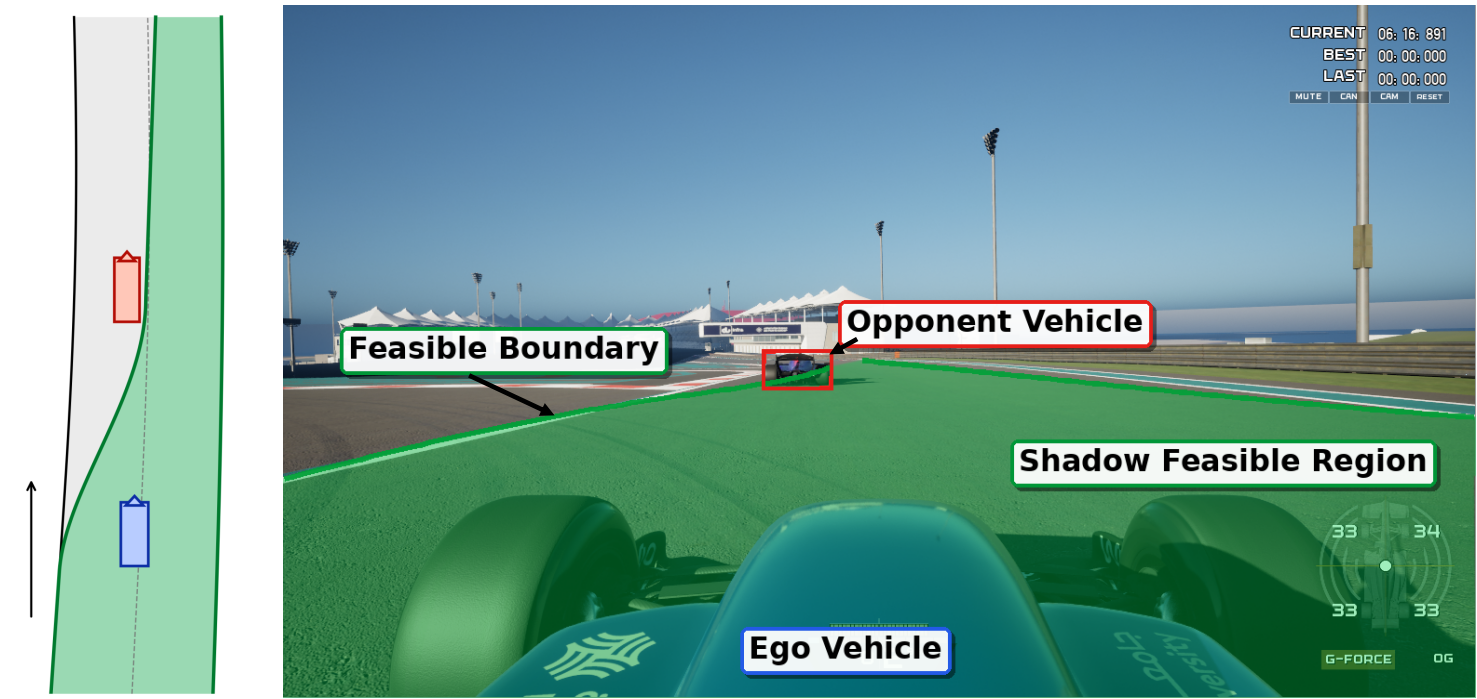
\includegraphics[width=0.48\linewidth]{shadow.png}}\\[-1mm]
\subfloat[\textsc{Overtake}.]{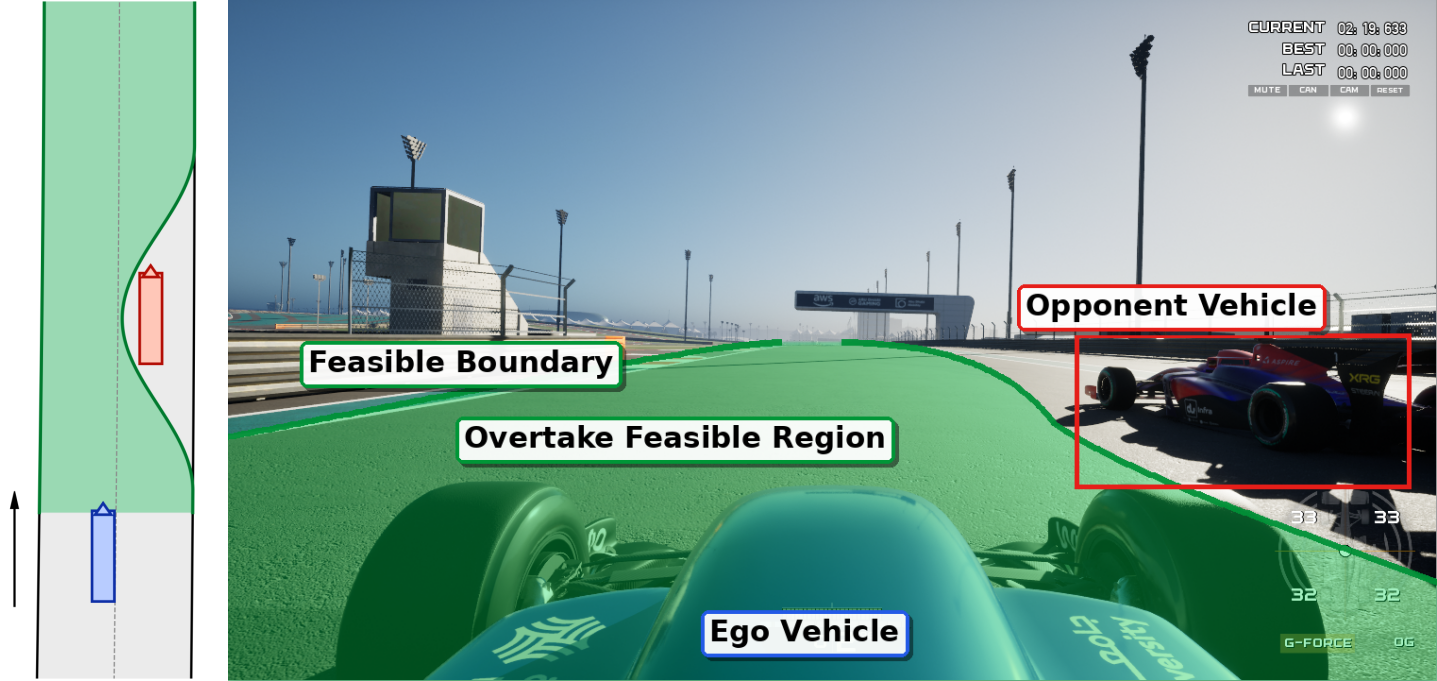
\includegraphics[width=0.48\linewidth]{overtake.png}}
\hfill
\subfloat[\textsc{Defend}.]{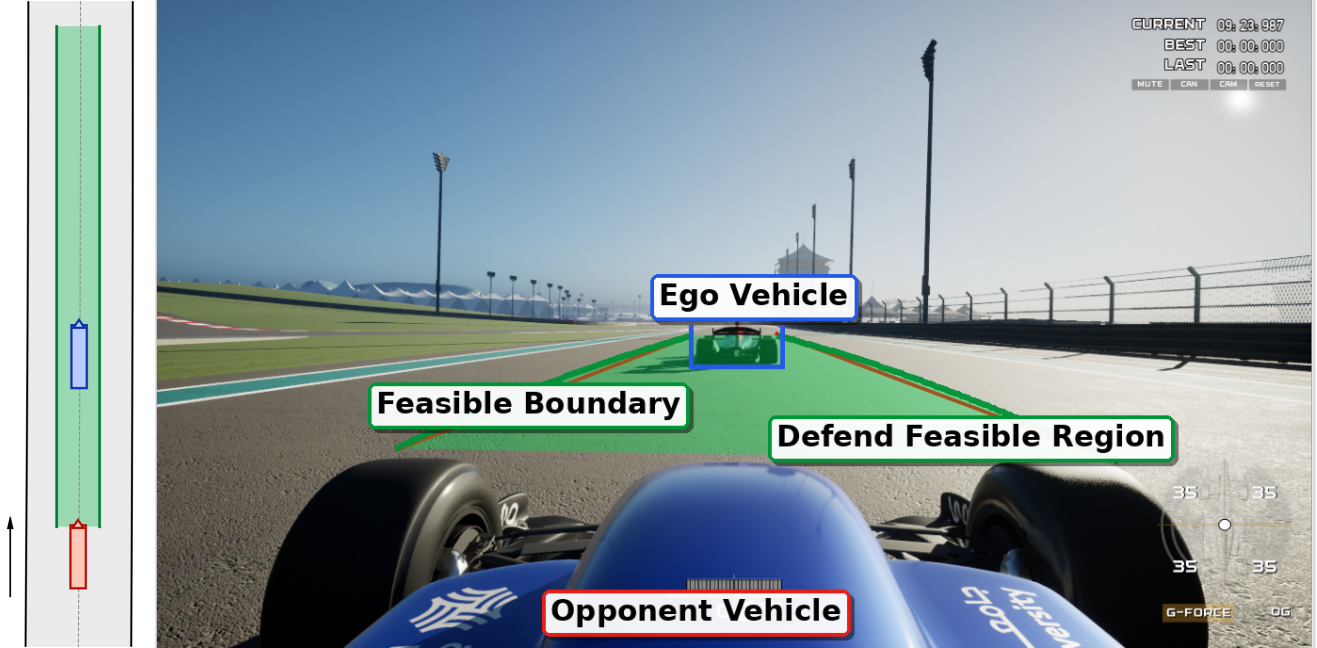
\includegraphics[width=0.48\linewidth]{defend.png}}
\caption{Geometric semantics of the persistent modes. Green regions are the
published feasible corridors. \textsc{Shadow} prepares the locked side,
\textsc{Overtake} excludes the opponent footprint on that side, and
\textsc{Defend} reserves the blocking corridor; the common executor receives
only the resulting bounds and speed cap.}
\label{fig:tactical_mode_semantics}
\end{figure}

This separation is the planner-facing interface of the method: a noisy or late
policy update cannot command an actuator directly. An inadmissible sample is
projected, a collapsed corridor is rejected, and a missing tactical update
holds the last feasible guidance for one control cycle.

% =====================================================================
\section{Corridor-Constrained Closed-Loop Execution}
\label{sec:execution}\label{sec:planner}\label{sec:controller}
% =====================================================================

The execution layer is common to the proposed method, every baseline, and
every ablation. It is specified here because the tactical corridor is meaningful
only if it can be converted into a closed-loop vehicle response, but it is not
claimed as a separate contribution. At stations $s_k$, the published bounds
are intersected with the track to obtain
$\underline n_k=\max(n^-_{t,k},n^-_{\rm trk,k})$ and
$\overline n_k=\min(n^+_{t,k},n^+_{\rm trk,k})$. With
$\bm z_k=[n_k,\xi_k]^\top$, sequential iteration $j$ linearizes
Eq.~\eqref{eq:spatial_model} as
$\widehat{\bm f}_{s,k}^{j}=\bm A_k^j\bm z_k+\bm B_k^j\omega_k+\bm b_k^j$
and imposes the trapezoidal spatial dynamics
\begin{equation}
\bm z_{k+1}-\bm z_k=\frac{\Delta s_{\rm sta}}{2}
\left[\widehat{\bm f}_{s,k}^{j}(\bm z_k,\omega_k)
+\widehat{\bm f}_{s,k+1}^{j}(\bm z_{k+1},\omega_{k+1})\right].
\label{eq:execution_spatial_dynamics}
\end{equation}
The path is the solution of the second-order cone program
\begin{equation}
\begin{aligned}
\bm y^{j+1}=\argmin_{\bm y}\;&
\sum_{k=0}^{N-1}w_\omega\sigma_k^\omega
+w_{n,T}\epsilon_n+w_{\xi,T}\epsilon_\xi\\
\mathrm{s.t.}\;&\bm z_0=[n_e,\xi_e]^\top,
\quad \text{Eq.~\eqref{eq:execution_spatial_dynamics}},\\
&\underline n_k\le n_k\le\overline n_k,\quad
\left\|[2\omega_k,\;\sigma_k^\omega-1]^\top\right\|_2
\le\sigma_k^\omega+1,\\
&|n_{N-1}-n_T|\le\epsilon_n,\quad
|\xi_{N-1}-\xi_T|\le\epsilon_\xi,\quad
\epsilon_n,\epsilon_\xi\ge0,
\end{aligned}
\label{eq:execution_socp}
\end{equation}
where $\bm y=\{\bm z_k,\omega_k,\sigma_k^\omega,\epsilon_n,
\epsilon_\xi\}$ and $n_T$ is the raceline or corridor midpoint selected by
the persistent mode. The cone is the epigraph of $\omega_k^2$; hence the cost
regularizes curvature while the terminal slack prevents numerical infeasibility
in a short, tightly carved corridor.

After reconstructing the Cartesian path, let
$\kappa_{p,k}\simeq\omega_k^\star$ and let $a_{T,k}^{+}(V)$ and
$b_{T,k}^{-}(V)>0$ denote the available propulsion and braking magnitudes after
applying Eqs.~\eqref{eq:tire_force_tangent} and~\eqref{eq:drag}. The curvature
ceiling and forward--backward sweep are
\begin{equation}
\begin{aligned}
\overline V_{{\rm lim},k}&=
\begin{cases}
v_{x,\max},&|\kappa_{p,k}|<\varepsilon_\kappa,\\
\displaystyle\lim_{r\to\infty}V_k^{(r)},&\text{otherwise},
\end{cases}\\[-1mm]
V_k^{(r+1)}&=\min\!\left\{v_{x,\max},
\sqrt{\frac{a_N^{\max}(V_k^{(r)})}{|\kappa_{p,k}|}}\right\},
\quad V_k^{(0)}=v_{x,\max},\\
V_{{\rm lim},k}&=\min\{\overline V_{{\rm lim},k},V_{{\rm cap},t}\},\\
\textcolor{blue}{V_0^f}
&\textcolor{blue}{=\operatorname{clip}_{[V_{\min},V_{{\rm lim},0}]}(V_e),}\\
V_{k+1}^{f}&=\operatorname{clip}_{[V_{\min},V_{{\rm lim},k+1}]}
\sqrt{(V_k^f)^2+2\Delta\ell_k a_{T,k}^{+}(V_k^f)},\\
\textcolor{blue}{V_{N-1}^b}
&\textcolor{blue}{=\min\{V_{N-1}^f,V_{{\rm lim},N-1}\},}\\
V_{k}^{b}&=\operatorname{clip}_{[V_{\min},V_{{\rm lim},k}]}
\sqrt{(V_{k+1}^b)^2+2\Delta\ell_k b_{T,k+1}^{-}(V_{k+1}^b)},\\
V_k^\star&=\min\{V_k^f,V_k^b,V_{{\rm lim},k}\}.
\end{aligned}
\label{eq:execution_speed_sweep}
\end{equation}
The curvature ceiling is evaluated by fixed-point iteration; the subsequent
passes enforce reachable acceleration and braking on the optimized path. The resulting
path--speed sequence is resampled at the controller period $T_c$.
\textcolor{blue}{The forward pass is anchored at the measured ego speed after
applying the local admissible bounds, whereas the backward pass starts from
the reachable terminal speed delivered by the forward pass.}

\textcolor{red}{For the MPCC, define
$\bm\chi_k=[x_k,y_k,\theta_k]^\top$ and
$\bm\nu_k=[V_k,\delta_k]^\top$.}
\textcolor{blue}{The fixed executor employs a reference-conditioned
contouring-error model predictive controller, referred to as MPCC hereafter
for consistency. Unlike progress-maximizing MPCC formulations that introduce
an additional virtual path-progress state, the deployed controller tracks the
time-resampled path--speed reference on a fixed prediction grid through
contouring-error, heading-error, speed-reference, and steering-reference
penalties. Its state and input are
$\bm\chi_k=[x_k,y_k,\theta_k]^\top$ and
$\bm\nu_k=[V_k,\delta_k]^\top$, respectively.}
Its identified local prediction model and the
principal tracking errors are
\begin{equation}
\begin{aligned}
\bm\chi_{k+1}&=\bm\chi_k+T_c
\begin{bmatrix}V_k\cos\theta_k&V_k\sin\theta_k&
\Omega(V_k,\delta_k)\end{bmatrix}^{\!\top},\\
\Omega(V,\delta)&=\frac{\tan(a_\delta\delta+b_\delta)}{L_c}(c_VV+d_V),\\
e_{c,k}&=(\bm n_k^r)^\top
\bigl([x_k-x_k^r,\;y_k-y_k^r]^\top\bigr),\quad
e_{\psi,k}=\operatorname{wrap}(\theta_k-\theta_k^r).
\end{aligned}
\label{eq:execution_mpcc_model}
\end{equation}
With $\bm e_{\nu,k}=\bm\nu_k-\bm\nu_k^r$, the receding-horizon problem is
\begin{equation}
\begin{aligned}
\min_{\{\bm\nu_k\}}\;&q_{\Delta\delta}(\delta_0-\delta_{-1})^2
+\sum_{k=0}^{N_c-1}\!\left(q_ce_{c,k+1}^2+q_\psi e_{\psi,k+1}^2
+\bm e_{\nu,k}^\top\bm R_\nu\bm e_{\nu,k}\right)\\
\mathrm{s.t.}\;&\text{Eq.~\eqref{eq:execution_mpcc_model}},\quad
V_{\min}\le V_k\le v_{x,\max},\quad |\delta_k|\le\delta_{\max},\\
&|V_k-V_{k-1}|\le\Delta V_{\max},\quad
|\delta_k-\delta_{k-1}|\le\dot\delta_{\max}T_c.
\end{aligned}
\label{eq:execution_mpcc}
\end{equation}
Only the first command is applied. The allocator then maps its longitudinal
request and steering angle to throttle, brake pressure, steering-actuator
position, and gear.

\begin{algorithm}[!tbp]
\caption{Common corridor-constrained executor}
\label{alg:executor}
\begin{algorithmic}[1]
\REQUIRE guidance $\mathcal G_t$, state $\bm x_t$, track model, previous path
\STATE Intersect tactical and track bounds; warm-start the previous path
\FOR{at most five sequential linearization iterations}
  \STATE form Eq.~\eqref{eq:execution_spatial_dynamics} and solve
  SOCP~\eqref{eq:execution_socp}; update the linearization path
\ENDFOR
\STATE reconstruct the Cartesian path and run
Eq.~\eqref{eq:execution_speed_sweep} under $V_{\rm cap}$
\STATE resample the path--speed reference and solve
MPCC~\eqref{eq:execution_mpcc}; invoke fallback on a failed health gate
\STATE map the first
\textcolor{red}{acceleration/steering}
\textcolor{blue}{speed/steering}
command to throttle, brake,
steering actuator, and gear; transmit through CAN
\RETURN actuator command and feasibility/health status
\end{algorithmic}
\end{algorithm}

Thus the proposed method changes the persistent feasible region and speed cap
supplied to a fixed executor, not the executor itself. In
Section~\ref{sec:experiments}, the corridor/path, mode, and tracking panels test
whether the game-layer decision persists and is executed; tire-force-envelope
utilization provides the subordinate dynamic-admissibility check.
